\documentclass[12pt, a4paper]{article}
\usepackage{graphicx}
\usepackage[top=1.6cm, bottom=1.6cm, left=2cm, right=2cm]{geometry}
\usepackage{ragged2e} % per \justify
\usepackage{tocloft} % Per personalizzare il ToC
\usepackage[framed,numbered,autolinebreaks,useliterate]{mcode}

\title{\Huge Prestazioni Modulazioni}
\author{Francesco Musto 0612707371 \\ Andrea Savastano 0612707904 \\ Mario Zito 0612708073}
\date{\today}



\begin{document}
	\maketitle
	\vspace{-1cm}
	\tableofcontents
	
	
	\newpage
	\section{Costellazioni Modulazioni}
	Delle 4 modulazioni prese in esame nelle simulazioni (PSK, PAM, QAM, PPM) ne vengono stampate le costellazioni, ove possibile, nel caso di M=16 ed \(E_{av}\)=1.
	\begin{figure}[ht]
		\centering
		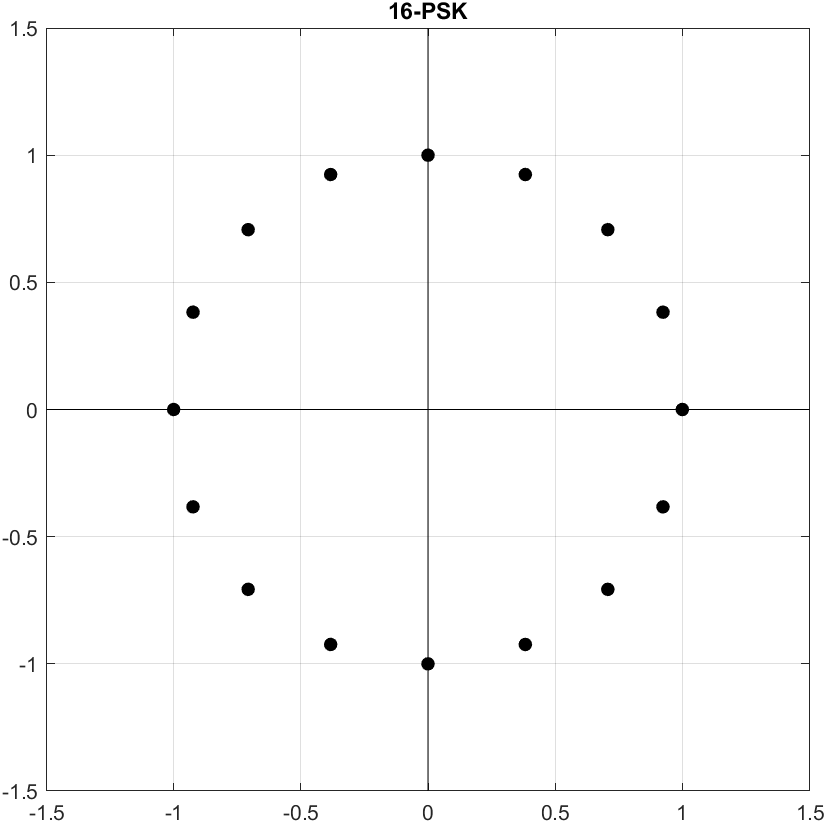
\includegraphics[width=0.35\linewidth]{images/16-PSK.png}
		\caption{16-PSK}
		\label{fig:psk}
		\begin{minipage}{0.45\linewidth} % Imposto la larghezza della mini pagina
			\centering
			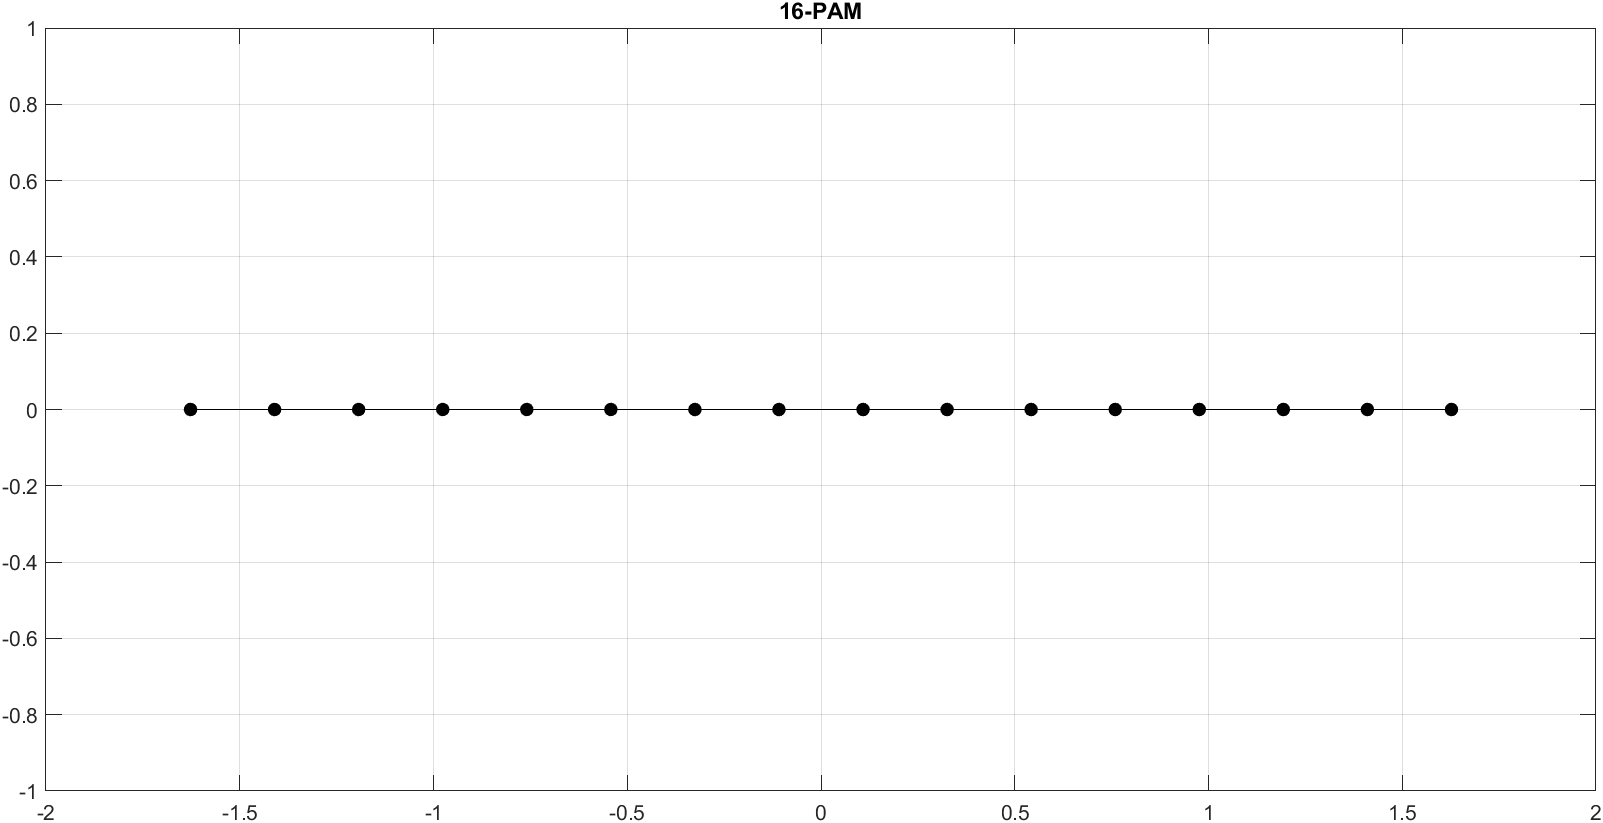
\includegraphics[width=\linewidth]{images/16-PAM.png}
			\caption{16-PAM}
			\label{fig:pam}
		\end{minipage}
		\hspace{0.5cm} % Spazio orizzontale tra le immagini
		\begin{minipage}{0.45\linewidth}
			\centering
			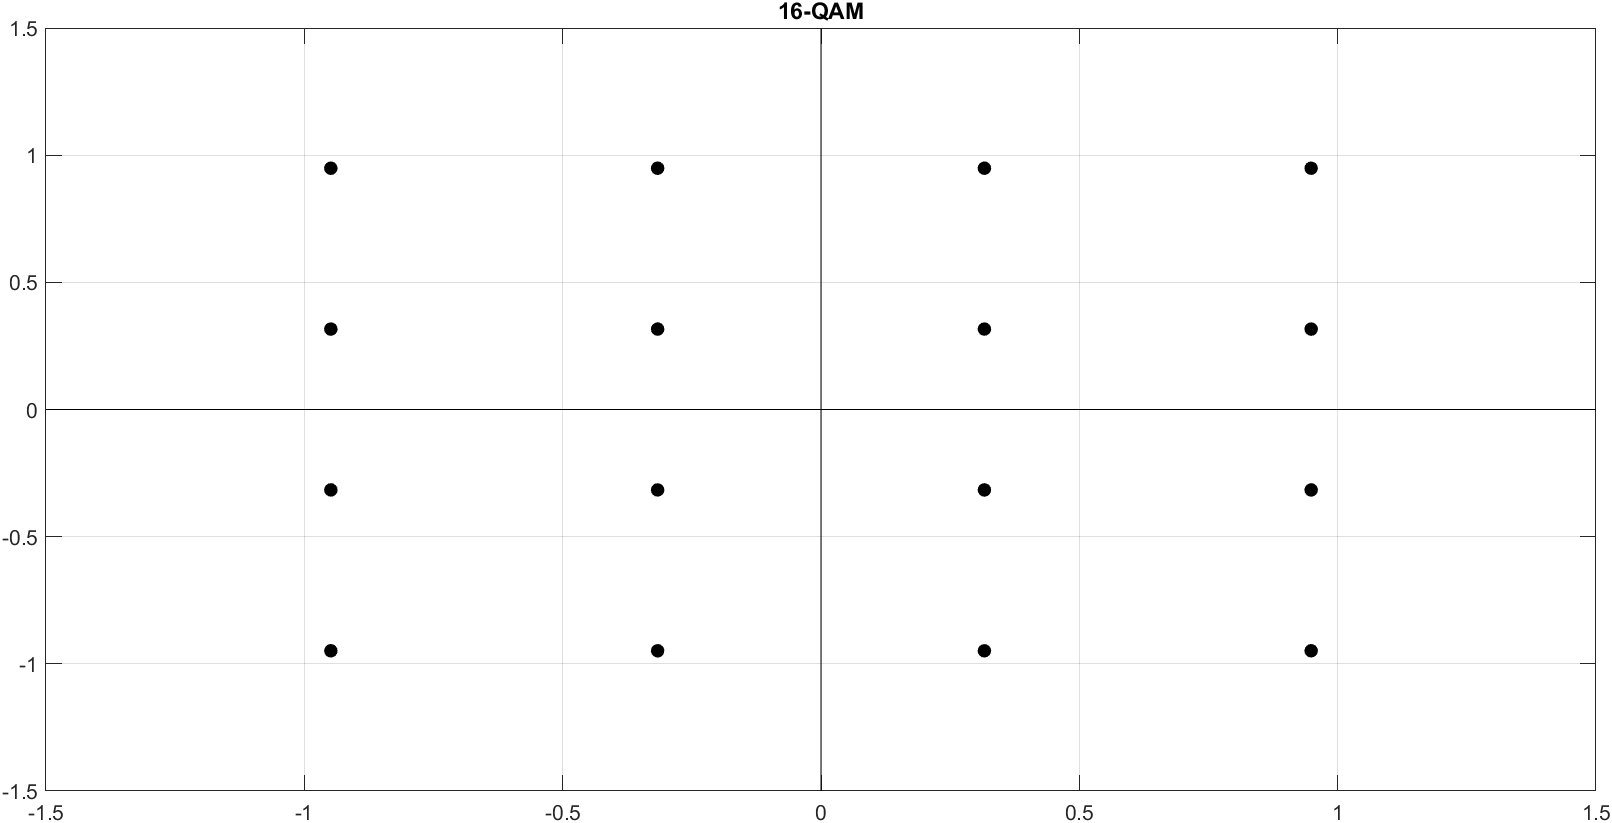
\includegraphics[width=\linewidth]{images/16-QAM.png}
			\caption{16-QAM}
			\label{fig:qam}
		\end{minipage}
	\end{figure}
	
	\subsection{Costellazioni con segnali ricevuti}
	Prendendo in considerazione le modulazioni PSK e QAM con M=8, \(E_{av}\)=1, \(SNR_{dB}\)=[10:20] e 50 prove MonteCarlo, ne vengono stampate le costellazioni con i segnali ricevuti in rosso. 
	\begin{figure}[ht]
		\begin{minipage}{0.4\linewidth} % Imposto la larghezza della mini pagina
			\centering
			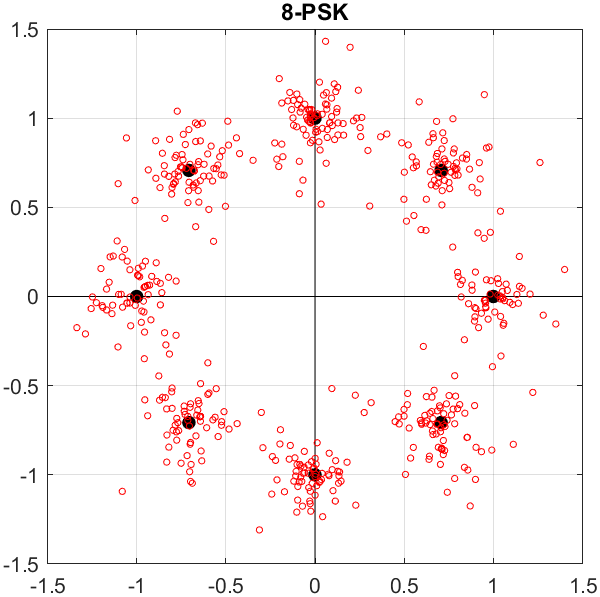
\includegraphics[width=\linewidth]{images/untitled2.png}
			%\caption{8-PSK}
			\label{fig:8-PSK}
		\end{minipage}
		\hspace{3cm} % Spazio orizzontale tra le immagini
		\begin{minipage}{0.4\linewidth}
			\centering
			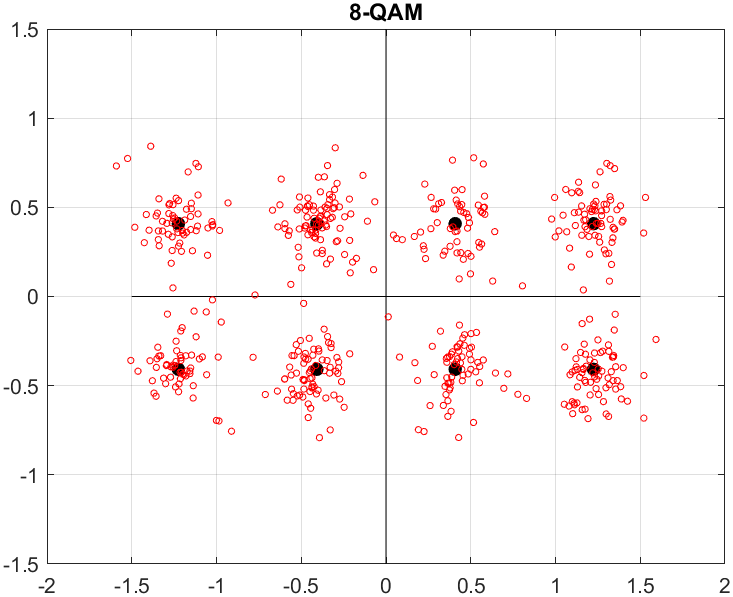
\includegraphics[width=\linewidth]{images/untitled1.png}
			%\caption{8-QAM}
			\label{fig:8-QAM}
		\end{minipage}
	\end{figure}
	\\Si noti che i segnali ricevuti si trovano vicino a quelli teorici, grazie all'\(SNR_{dB}\) alto.
	
	
	
	\newpage
	\section{Confronto PAM - PPM}
	\subsection{2-PAM con 2-PPM}
	Simulazione delle modulazioni 2-PAM e 2-PPM con \(SNR_{dB}\)=[-10:15], \(10^5\) prove MonteCarlo. \vspace{.1cm}\\
	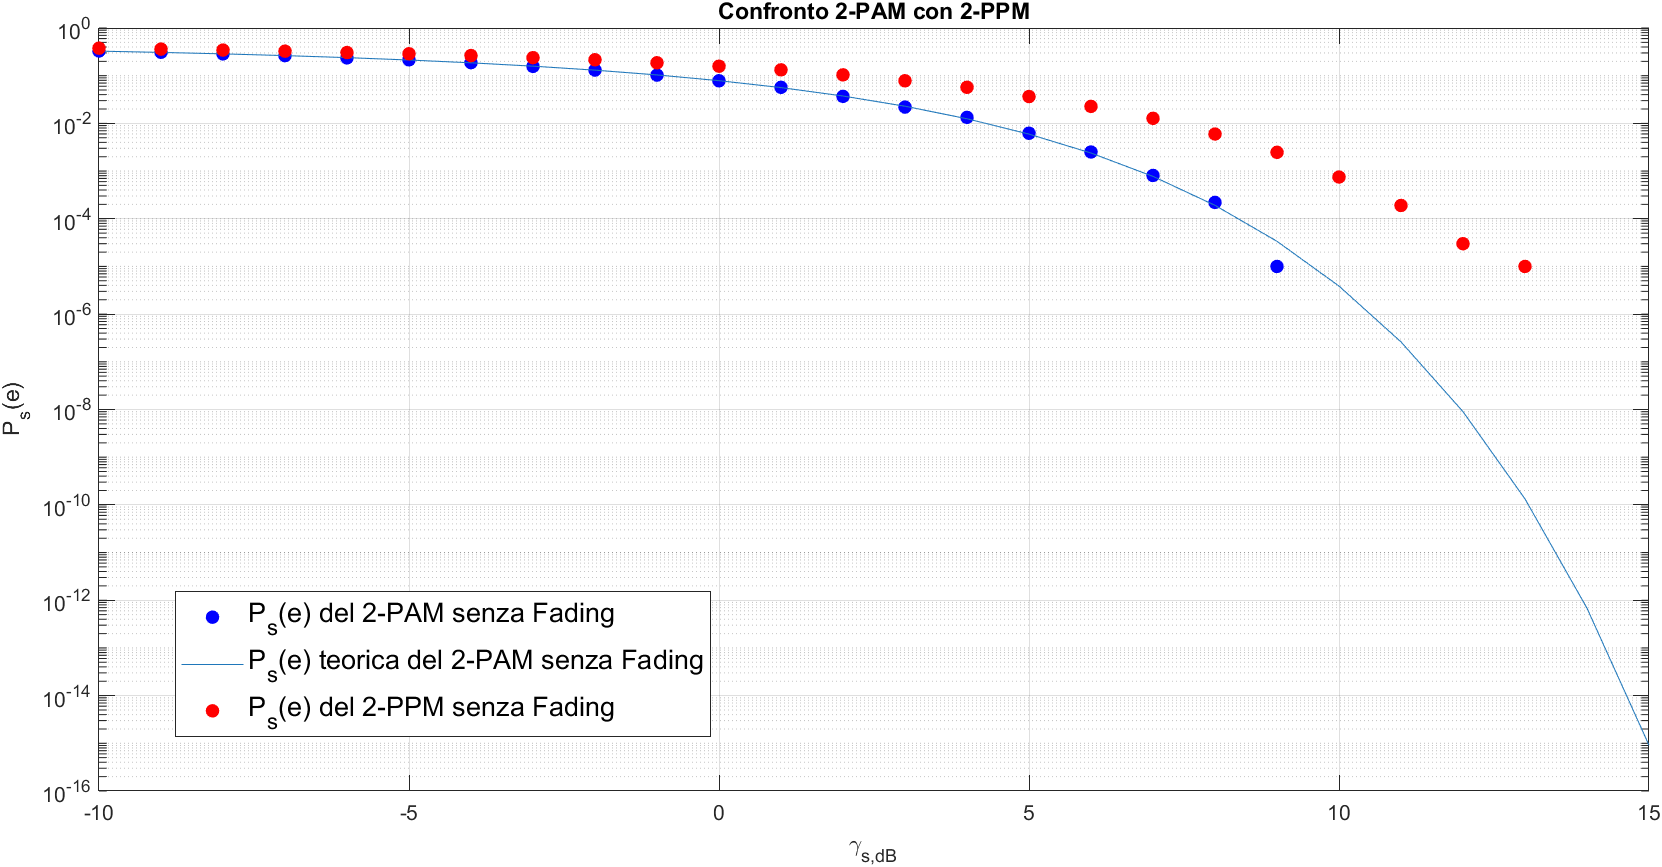
\includegraphics[width=\linewidth]{images/2-PAMvs2-PPM.png}
	In questa prima simulazione la curva blu, relativa alle prestazioni del 2-PAM, decresce più velocemente rispetto alla curva rossa del 2-PPM, al crescere dell'\(SNR_{dB}\). Questo dimostra che per il numero di bit scelto (k=2), il PAM risulta più prestante del PPM.
	\subsection{16-PAM con 16-PPM}
	Simulazione delle modulazioni 16-PAM e 16-PPM con \(SNR_{dB}\)=[-10:30], \(10^5\) prove MonteCarlo. \\
	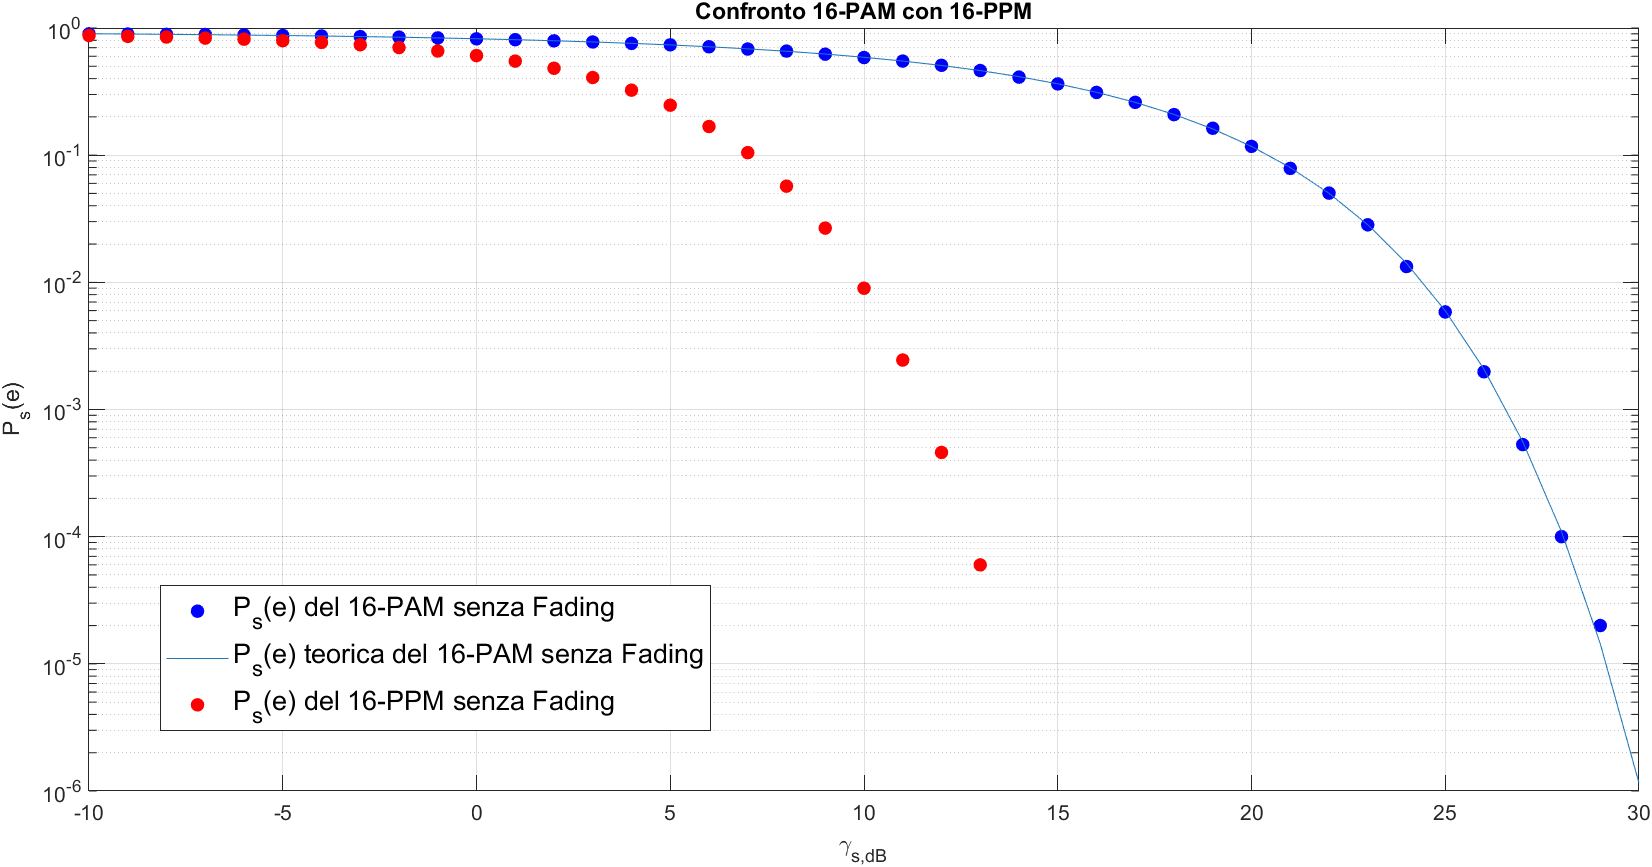
\includegraphics[width=\linewidth]{images/PAMvsPPM.png}
	Rispetto alla simulazione precedente, il PPM risulta molto più prestante del PAM per il numero di bit scelto (k=4). Se si continuasse ad aumentare il numero k di bit in ulteriori simulazioni, si noterebbe che le prestazioni del PAM continuerebbero a peggiorare, mentre quelle del PPM a migliorare. 
	
	
	
	\newpage
	\section{Prestazioni 16-QAM}
	Simulazione di una modulazione 16-QAM con \(SNR_{dB}\)=[-10:30], \(10^6\) prove MonteCarlo e L=2 ritrasmissioni\vspace{.1cm}\\
	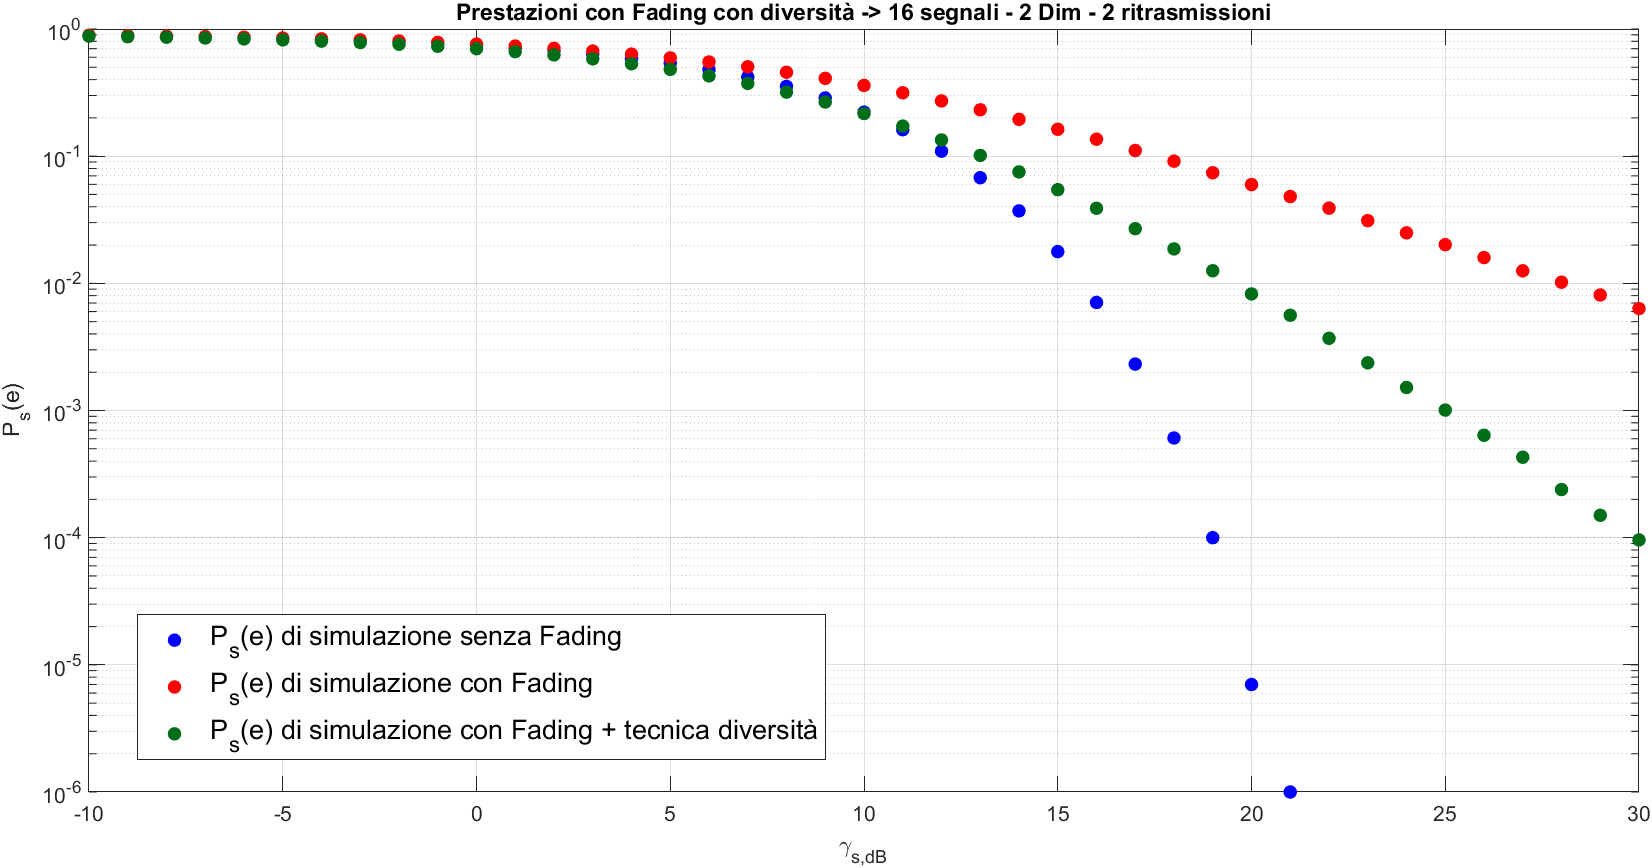
\includegraphics[width=\linewidth]{images/QAM MC 1e6.png}
	\subsection{Senza Fading}
	La curva azzurra mostra come la \(P_s(e)\) decresce \underline{esponenzialmente} all’aumentare dell’SNR considerato.
	\subsection{Con Fading}
	La curva rossa mostra come la \(P_s(e)\) decresce \underline{iperbolicamente} (più lentamente) all’aumentare dell’SNR.\\
	Si noti come le prestazioni risultano pessime rispetto al caso in cui il Fading è assente.
	\subsection{Con Tecnica di Diversità in tempo/frequenza}
	La curva verde mostra come la \(P_s(e)\) decresce in maniera più veloce rispetto a quella in presenza di Fading.\\
	Utilizzando L=2 ritrasmissioni si riesce a fronteggiare il Fading, ottenendo delle prestazioni tollerabili.
	
	
	\newpage
	\section{Prestazioni 16-PSK al variare di L}
	Simulazione di una modulazione 16-PSK con \(SNR_{dB}\)=[-10:30], \(10^5\) prove MonteCarlo e ripetuta due volte: la prima con un numero L di ritrasmissioni pari a 2 e la seconda con L=5.
	\subsection{L=2}
	\centering
	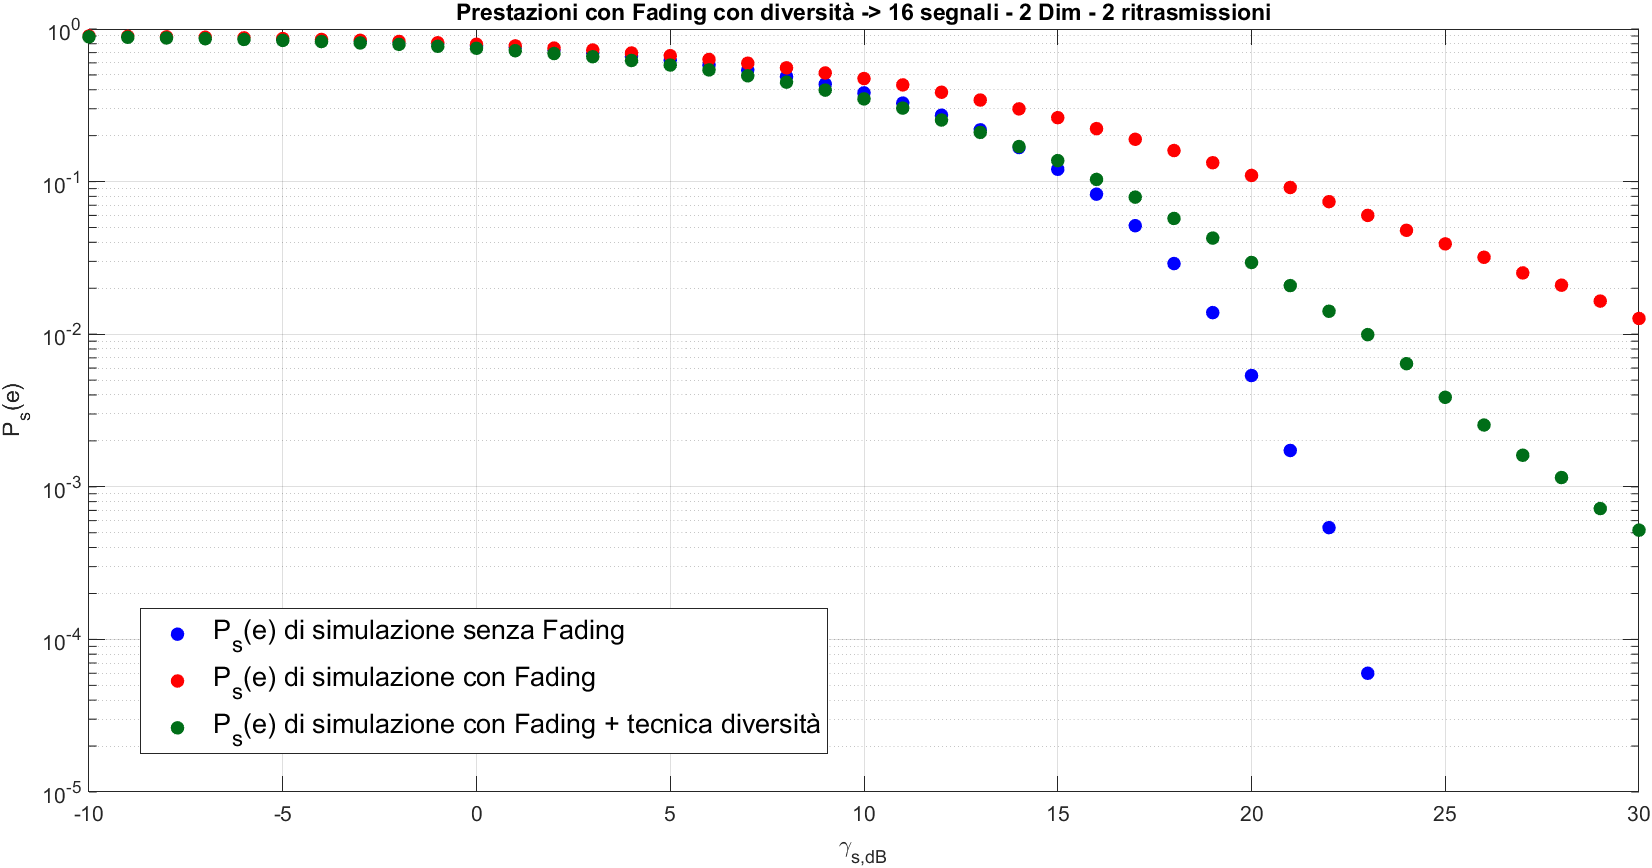
\includegraphics[width=0.85\linewidth]{images/PSK 1e5 2 L.png}
	\justify
	\subsection{L=5}
	\centering
	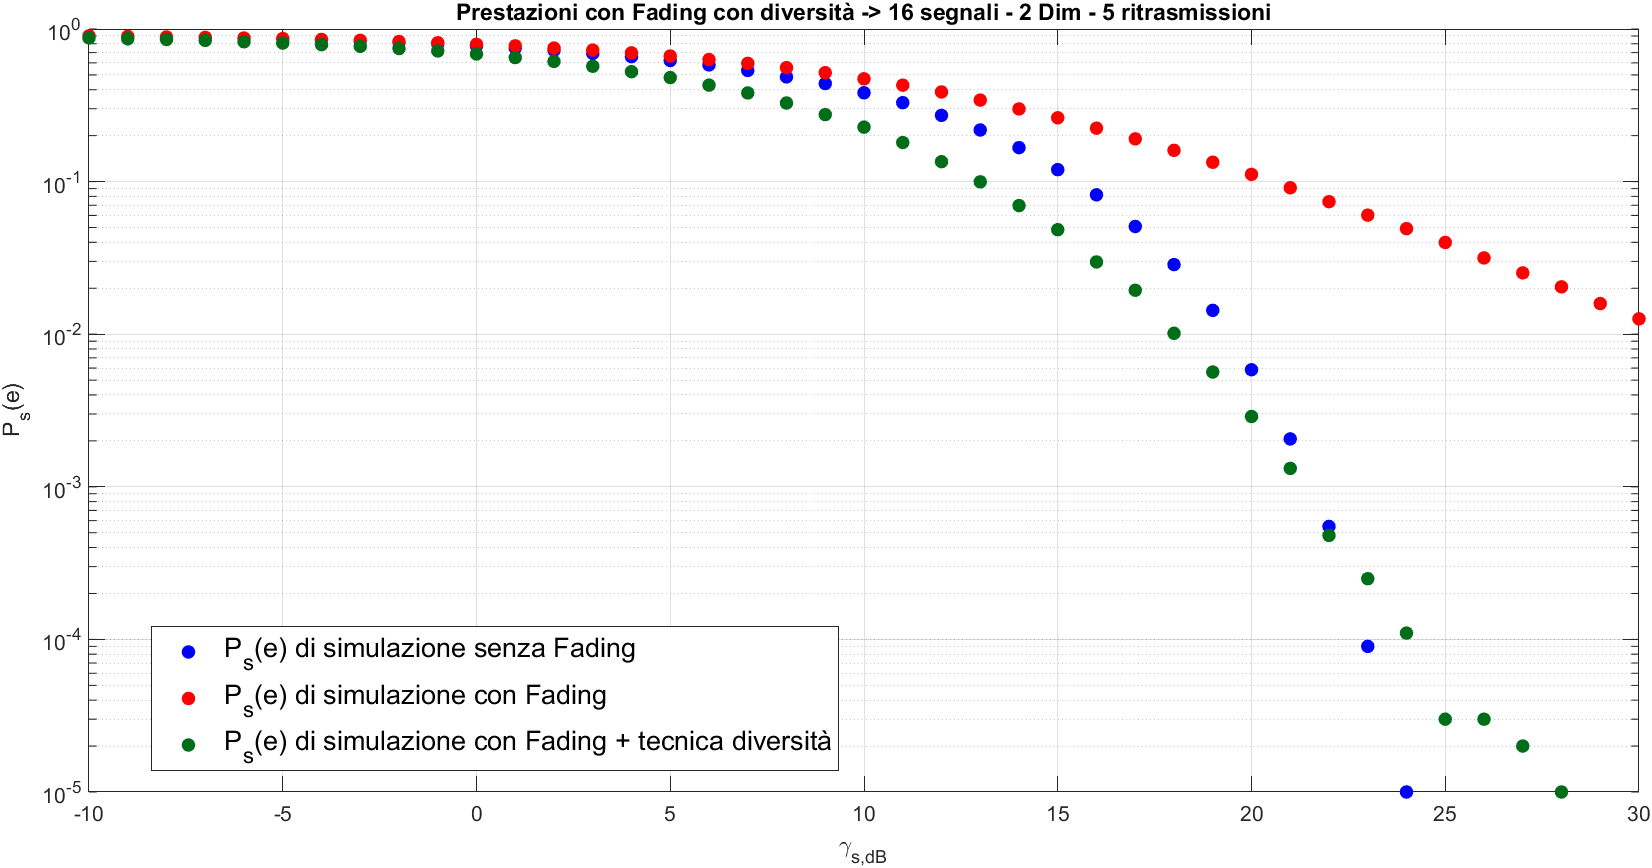
\includegraphics[width=0.85\linewidth]{images/PSK 1e5 5 L.png}
	\justify
	Confrontando le curve verdi e blu dei 2 grafici è possibile notare che all’aumentare delle ritrasmissioni (da L=2 a L=5) le prestazioni migliorano in maniera significativa.\vspace{.3cm} \\
	Entrando nel dettaglio, all’aumentare dell’SNR, la \(P_s(e)\) nel primo grafico (L=2) segue inizialmente quella del caso senza Fading per poi allontanarsi da quest’ultima, rimanendo comunque al di sotto di quella con il Fading.\vspace{.3cm}\\
	Questo è dovuto al fatto che la tecnica di diversità scelta faccia selezionare tra le L=2 ritrasmissioni quella con maggiore SNR.\vspace{.3cm}\\
	Nel secondo grafico (L=5) si può notare che la \(P_s(e)\) si trova addirittura al di sotto di quella del caso in cui il fenomeno del Fading non è considerato; sinonimo del fatto che le prestazioni sono migliorate ancor di più.
	
	
	\newpage
	\section{Prestazioni 8-PPM al variare di MC}
	Simulazione di una modulazione 8-PPM con \(SNR_{dB}\)=[-10:30], L=2 e ripetuta due volte: \\la prima con un numero MonteCarlo di prove pari a \(10^4\) e la seconda con MC=\(10^6\).
	\subsection{MC=\(10^4\)}
	\centering
	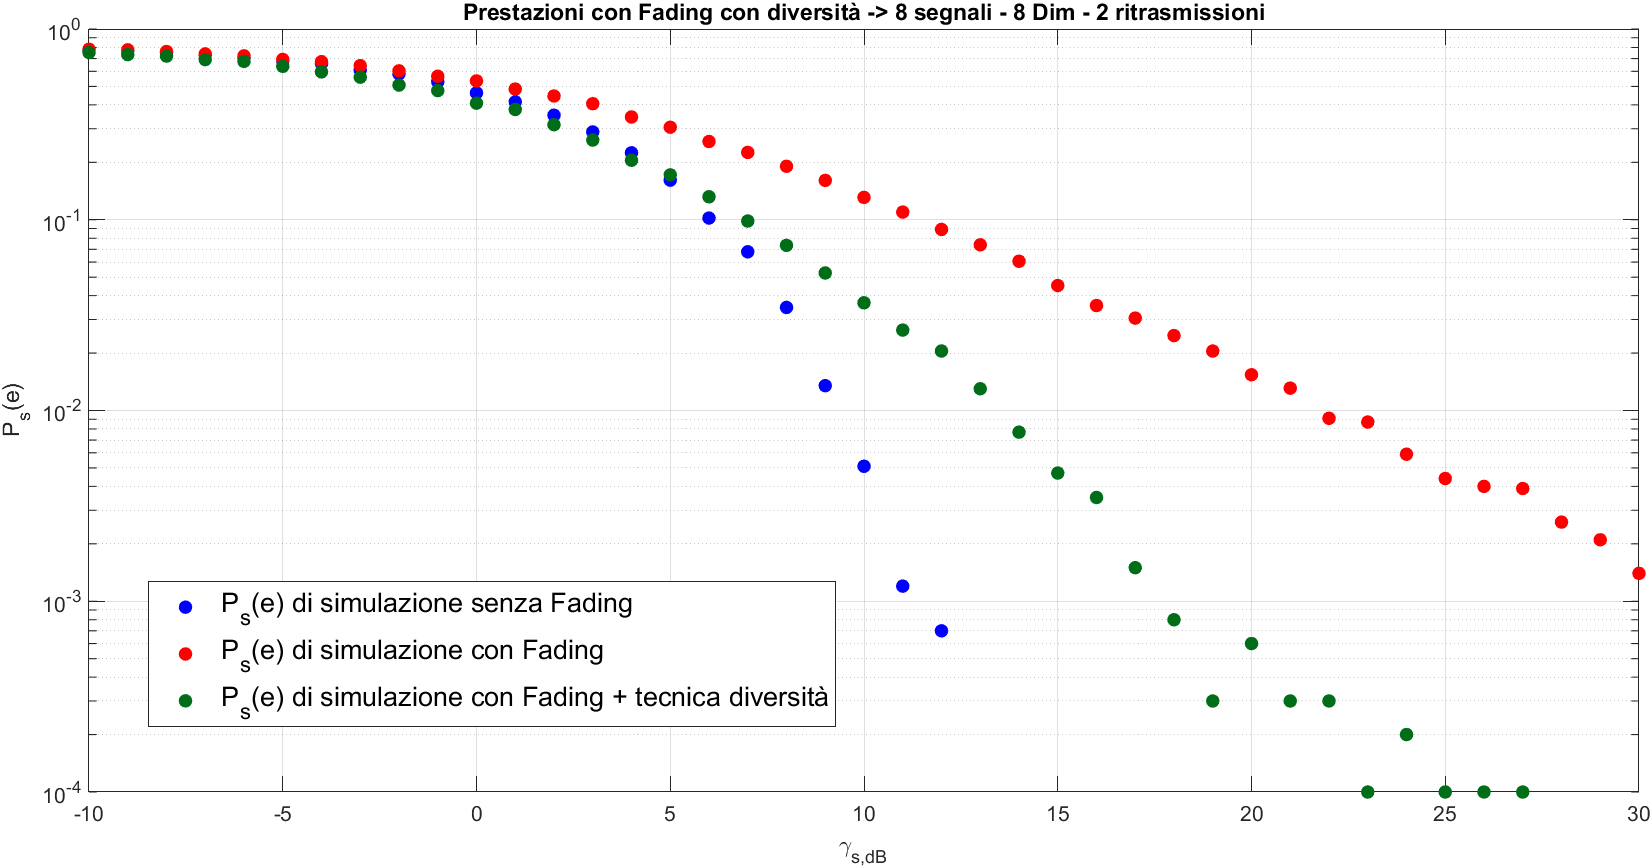
\includegraphics[width=0.85\linewidth]{images/MC_104.png}
	\justify
	\subsection{MC=\(10^6\)}
	\centering
	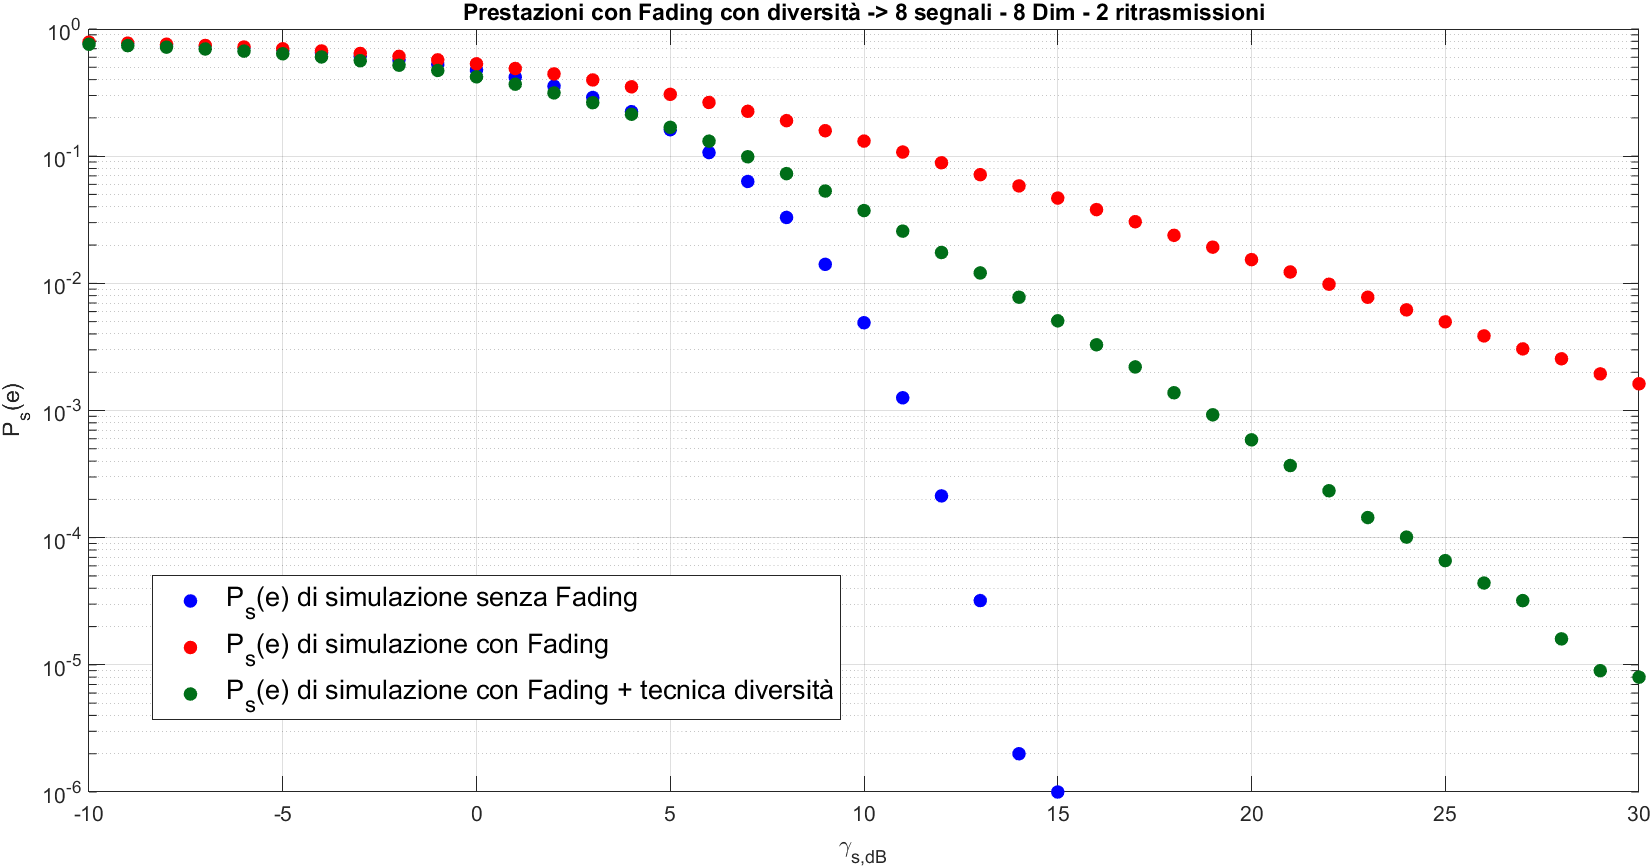
\includegraphics[width=0.85\linewidth]{images/MC_106.png}
	\justify
	Osservando la prima figura (MC=\(10^4\)), la curva azzurra non presenta stime precise della \(P_s(e)\) per valori di \(SNR_{dB}\) più alti, in particolare da \(SNR_{dB}\)=10 fino a 30. 
	\\Questo è dovuto al numero insufficiente di prove MC, sulle quali è stata stimata una \(P_s(e)\)=0 per gli \(SNR_{dB}\) alti. In questo caso la \(P_s(e)\) non si può mostrare perchè è in scala logaritmica.
	\vspace{.3cm}\\Invece per la curva rossa vengono mostrate le stime della \(P_s(e)\) per ogni \(SNR_{dB}\) perchè, in presenza del Fading (SNR come variabile aleatoria esponenziale), l'SNR effettivo è minore e questo facilita la stima della \(P_s(e)\), perchè vi sono più errori.
	\vspace{.3cm}\\Osservando la seconda figura (MC=\(10^6\)), la curva azzurra presenta stime più precise della \(P_s(e)\), fornendone una fino a \(SNR_{dB}\)=15. Dopo questo valore, anche in questo caso, non è possibile ottenere stime della \(P_s(e)\) perchè il numero MC di prove risulta ancora insufficiente.
	
	
	
	
	\newpage
	\section{Resoconto finale}
	Per effettuare un'analisi complessiva delle simulazioni, si evince che un aumento del rapporto segnale-rumore (SNR) nelle trasmissioni conduce a un miglioramento delle prestazioni. 
	\\Tuttavia, tale incremento risulta insufficiente per ottenere prestazioni accettabili in presenza di Fading, rendendo pertanto necessaria l'introduzione di almeno una tecnica di diversità. Quella implementata nelle simulazioni prevede la ritrasmissione dello stesso segnale, consentendo di migliorare le prestazioni anche in condizioni di Fading.
	
	\vspace{2cm}
	\appendix
	\addtocontents{toc}{\vspace{.5cm}} % Aggiunge uno spazio prima dell'appendice
	\section*{Appendice: Codice Matlab}
	\addcontentsline{toc}{section}{Appendice: Codice Matlab} % Aggiunge l'appendice al ToC
	
	\section{Main}
	\begin{lstlisting}
		function proj_main(Str, k, SNRdB, MC, flag, L)
		%% parametri In
		% --INPUT--
		% Str:   e' la modulazione da utilizzare 
		% k:     numero di bit da trasmettere
		% SNRdB: Rapporto segnale rumore per decibel per simbolo
		% MC:    numero MonteCarlo di trasmissioni per ogni SNR
		% flag:  a 1 per simulare il Fading
		% L:     numero di ritrasmissioni per la tecnica di diversita' (flag=1)
		
		%% Controllo
		if k==0
		fprintf('k deve essere maggiore di 0\n')
		return;
		end
		
		%% Scelta modulazione
		if strcmpi(Str,'PAM')
		Cost = proj_PAM_generator(k);    
		elseif strcmpi(Str,'PPM')
		Cost = proj_PPM_generator(k);
		elseif strcmpi(Str,'PSK')
		Cost = proj_PSK_generator(k);
		elseif strcmpi(Str,'QAM')
		Cost = proj_QAM_generator(k);
		else
		fprintf('Str deve essere PAM / PPM / PSK / QAM \n')
		return;
		end
		
		%% Simulazione con o senza Fading
		proj_estimate_Pe(SNRdB, Cost, MC);
		if flag
		proj_estimate_Pe_Fading(SNRdB, Cost, MC);
		if L>1
		proj_estimate_Pe_diversity(SNRdB, Cost, MC, L);
		end
		end
	\end{lstlisting}
	
	\newpage
	\section{Generatore costellazioni}
	\subsection{Generatore PAM}
	\begin{lstlisting}
		function Cost = proj_PAM_generator(k)
		%% parametri In-Out
		% --INPUT--
		% k:     numero di bit da trasmettere
		
		% --OUTPUT--
		% Cost:  Costellazione dei segnali in forma matriciale -> Mx1 (PAM)
		
		%% calcolo matrice Cost
		M = 2^k;
		Am = linspace(-(M-1), M-1, M);
		Eg = 3/(M^2-1);
		Cost = (Am*sqrt(Eg))';
		
		%% stampa costellazione PAM
		plot(Cost,zeros(1,M),'ko-','MarkerSize',6,'MarkerFaceColor','k')
		hold on
		title(M+'-PAM')
		grid on
	\end{lstlisting}
	\subsection{Generatore QAM}
	\begin{lstlisting}
		function Cost = proj_QAM_generator(k)
		%% parametri In-Out
		% --INPUT--
		% k:     numero di bit da trasmettere
		
		% --OUTPUT--
		% Cost:  Costellazione dei segnali in forma matriciale -> Mx2 (QAM)
		
		%% calcolo matrice Cost
		M = 2^k;
		qam_symbols = qammod(0:M-1, M);
		Cost(:,1) = real(qam_symbols); 
		Cost(:,2) = imag(qam_symbols);
		
		Eav = sum(Cost(:,1).^2+Cost(:,2).^2)/M;
		Cost = Cost./sqrt(Eav);
		
		%% stampa costellazione PSK
		plot(Cost(:,1),Cost(:,2),'ko','MarkerSize',6,'MarkerFaceColor','k')
		hold on
		plot([-1.5 1.5],[0 0],'k-','MarkerSize',6,'MarkerFaceColor','k')
		plot([0 0],[-1.5 1.5],'k-','MarkerSize',6,'MarkerFaceColor','k')
		title(M+'-QAM')
		grid on
	\end{lstlisting}
	\newpage
	\subsection{Generatore PSK}
	\begin{lstlisting}
		function Cost = proj_PSK_generator(k)
		%% parametri In-Out
		% --INPUT--
		% k:     numero di bit da trasmettere
		
		% --OUTPUT--
		% Cost:  Costellazione dei segnali in forma matriciale -> Mx2 (PSK)
		
		%% calcolo matrice Cost
		M = 2^k;
		D = M/2;
		Cost = zeros(M,2);
		
		% Avendo posto Eav=1 i segnali sono equienergetici: Es=1 per ogni m --> r=1
		% quindi gli M segnali sono equidistanti dal centro della circonferenza (r=1)
		% sx ed sy sono le coordinate dei singoli segnali su x e su y e quindi 
		% gli elementi di ogni riga della costellazione Cost.
		for ii=1:M
		sx = cos(ii*pi/D);
		sy = sin(ii*pi/D);
		Cost(ii,1) = sx;
		Cost(ii,2) = sy;
		end
		
		%% stampa costellazione PSK
		plot(Cost(:,1),Cost(:,2),'ko','MarkerSize',6,'MarkerFaceColor','k')
		hold on
		plot([-1.5 1.5],[0 0],'k-','MarkerSize',6,'MarkerFaceColor','k')
		plot([0 0],[-1.5 1.5],'k-','MarkerSize',6,'MarkerFaceColor','k')
		title(M+'-PSK')
		grid on
		axis('square')
	\end{lstlisting}
	\subsection{Generatore PPM}
	\begin{lstlisting}
		function Cost = proj_PPM_generator(k)
		%% parametri In-Out
		% --INPUT--
		% k:     numero di bit da trasmettere
		
		% --OUTPUT--
		% Cost:  Costellazione dei segnali in forma matriciale -> MxM (PPM)
		
		%% calcolo matrice Cost
		%tutti gli M segnali sono equienergetici e Es = 1 per ogni m
		%quindi Eav = = Esm = 1
		M = 2^k;
		Cost = eye(M); 
	\end{lstlisting}
	\newpage
	
	\section{Stima \(P_s(e)\)}
	\subsection{\(P_s(e)\) senza Fading}
	\begin{lstlisting}
		function Pe_s = proj_estimate_Pe(SNRdB, Cost, MC)
		%% parametri In-Out
		% --INPUT--
		% SNRdB: Rapporto segnale rumore per decibel per simbolo
		% Cost:  M righe = M regnali, N colonne = dimensionalita'
		% MC:    numero MonteCarlo di trasmissioni per ogni SNR
		
		% --OUTPUT--
		% Pe_s:  Probabilita' di errore per simbolo su MC prove e per diversi SNR
		
		%% parametri utili
		SNRnf = 10.^(SNRdB/10); % SNR no Fading per SIMBOLO
		Eav = 1; 
		N0 = Eav./SNRnf; % varia N0
		M = length(Cost(:,1));
		N = length(Cost(1,:));
		Pe_s = zeros(1,length(SNRnf));
		%% calcolo Ps(e)
		for ii=1:length(SNRnf)
		N0_now = N0(ii);
		errori = zeros(1,MC);
		for jj=1:MC        
		indexTx = randi(M);
		% scegliamo una delle M righe = una degli M segnali
		s = Cost(indexTx,:);
		r = s + randn(1,N)*sqrt(N0_now/2);
		
		% plot del segnale ricevuto
		% if N==1
		%     plot(r,0,'ro','MarkerSize',3);
		% elseif N==2
		%     plot(r(1),r(2),'ro','MarkerSize',3);
		% end
		
		% calcolo della minima distanza
		d_min = norm(r - Cost(1,:));
		indexRx = 1;
		for zz=2:M
		d_tmp = norm(r - Cost(zz,:));
		if(d_tmp < d_min)
		d_min = d_tmp;
		indexRx = zz;
		end           
		end
		
		errori(jj) = indexTx~=indexRx; 
		end
		Pe_s(ii) = mean(errori);
		end
		
		%% Stampa 
		figure 
		semilogy(SNRdB, Pe_s, 'bo', 'MarkerSize', 6, 'MarkerFaceColor', 'b')
		
		hold on
		title('Prestazioni Modulazione - '+M+' segnali - '+N+' Dim')
		xlabel('\gamma_{s,dB}')
		ylabel('P_s(e)')
		lgd = legend('P_s(e) di simulazione senza Fading');
		
		if N==1 % la modulazione e' il PAM
		% non mettiamo log2(M) perche' SNR e' gia' per simbolo
		Pe_s_th = 2*(M-1)/M * qfunc(sqrt(6/(M^2-1)*SNRnf));
		semilogy(SNRdB, Pe_s_th, 'Color','#1f77ba');
		lgd = legend('P_s(e) di simulazione senza Fading', ...
		'P_s(e) teorica senza Fading');
		end
		lgd.FontSize = 13; 
		grid on
	\end{lstlisting}
	\subsection{\(P_s(e)\) con Fading}
	\begin{lstlisting}
		function Pe_s = proj_estimate_Pe_Fading(SNRdB, Cost, MC)
		%% parametri In-Out
		% --INPUT--
		% SNRdB: Rapporto segnale rumore per decibel per simbolo
		% Cost:  M righe = M regnali, N colonne = dimensionalita'
		% MC:    numero MonteCarlo di trasmissioni per ogni SNR
		
		% --OUTPUT--
		% Pe_s:  Probabilita' di errore per simbolo su MC prove e per diversi SNR
		
		%% parametri utili
		SNRnom = 10.^(SNRdB/10);
		Eav = 1;
		M = length(Cost(:,1));
		N = length(Cost(1,:));
		Pe_s = zeros(1,length(SNRnom));
		%% calcolo Ps(e)
		for ii=1:length(SNRnom)
		errori = zeros(1,MC);
		for jj=1:MC
		SNRrv = myexprnd(SNRnom(ii),1,1);
		N0_now = Eav/SNRrv;
		
		indexTx = randi(M);
		s = Cost(indexTx,:);
		r = s + randn(1,N)*sqrt(N0_now/2);
		
		d_min = norm(r - Cost(1,:));
		indexRx = 1;
		for zz=2:M
		d_tmp = norm(r - Cost(zz,:));
		if(d_tmp < d_min)
		d_min = d_tmp;
		indexRx = zz;
		end           
		end
		
		errori(jj) = indexTx~=indexRx; 
		end
		Pe_s(ii) = mean(errori);
		end
		
		%% Stampa 
		semilogy(SNRdB, Pe_s, 'ro', 'MarkerSize', 6, 'MarkerFaceColor', 'r')
		
		title('Prestazioni con Fading '+M+' segnali - '+N+' Dim')
		lgd = legend('P_s(e) di simulazione senza Fading', ...
		'P_s(e) di simulazione con Fading');
		
		if N==1
		% Calcolo Pe teorica con Fading per il PAM
		Pe_s_th_F = zeros(1,length(SNRnom));
		for ii=1:length(SNRnom)
		Pe_s_th_F(ii) = (M-1)/M * (1-sqrt(1/(1+(M^2-1)/(3*SNRnom(ii))) ));
		end
		semilogy(SNRdB, Pe_s_th_F, 'Color', '#FF6506')
		lgd = legend('P_s(e) di simulazione senza Fading', ...
		'P_s(e) teorica senza Fading', ...
		'P_s(e) di simulazione con Fading', ...
		'P_s(e) teorica con Fading');
		end
		lgd.FontSize = 13;
	\end{lstlisting}
	\subsection{\(P_s(e)\) con Fading e tecnica diversità}
	\begin{lstlisting}
		function Pe_s = proj_estimate_Pe_diversity(SNRdB, Cost, MC, L)
		%% parametri In-Out
		% --INPUT--
		% SNRdB: Rapporto segnale rumore per decibel per simbolo
		% Cost:  M righe = M regnali, N colonne = dimensionalita'
		% MC:    numero MonteCarlo di trasmissioni per ogni SNR
		% L:     numero di ritrasmissioni per la tecnica di diversita'
		
		% --OUTPUT--
		% Pe_s:  Probabilita' di errore per simbolo su MC prove e per diversi SNR
		
		%% parametri utili
		SNRnom = 10.^(SNRdB/10);
		Eav = 1;
		M = length(Cost(:,1));
		N = length(Cost(1,:));
		Pe_s = zeros(1,length(SNRnom));
		%% calcolo Ps(e)
		for ii=1:length(SNRnom)
		errori = zeros(1,MC);
		for jj=1:MC
		indexTx = randi(M);
		s = Cost(indexTx,:);
		
		SNRrv = myexprnd(SNRnom(ii),1,L);        
		N0_now = Eav/max(SNRrv);        
		r = s + randn(1,N)*sqrt(N0_now/2);
		
		d_min = norm(r - Cost(1,:));
		indexRx = 1;
		for zz=2:M
		d_tmp = norm(r - Cost(zz,:));
		if(d_tmp < d_min)
		d_min = d_tmp;
		indexRx = zz;
		end           
		end
		
		errori(jj) = indexTx~=indexRx; 
		end
		Pe_s(ii) = mean(errori);
		end
		
		%% Stampa 
		semilogy(SNRdB, Pe_s, 'o','Color', '#006e18','MarkerSize', 6, 'MarkerFaceColor', '#006e18')
		
		title('Prestazioni con Fading con diversita' -> '+M+' segnali - '+N+' Dim - '+L+' ritrasmissioni')
		lgd = legend('P_s(e) di simulazione senza Fading', ...
		'P_s(e) di simulazione con Fading', ...
		'P_s(e) di simulazione con Fading + tecnica diversita'');
		
		if N==1
		lgd = legend('P_s(e) di simulazione senza Fading', ...
		'P_s(e) teorica senza Fading', ...
		'P_s(e) di simulazione con Fading', ...
		'P_s(e) teorica con Fading', ...
		'P_s(e) di simulazione con Fading + tecnica diversita'');
		end
		lgd.FontSize = 13;
	\end{lstlisting}
	\subsubsection{myexprnd ausiliaria}
	\begin{lstlisting}
		function y=myexprnd(mu,r,c)
		y=-mu*log(rand(r,c));
	\end{lstlisting}
	
\end{document}